\chapter{A mixture of experts online learning system}
\label{chap:mix_online_learning}

In this chapter, we continue our work on behavior prediction from chapter ~\ref{chap:behav_pred}.
Although the various models developed there show already promising results, they are intended to be trained offline and without any adaptation at run time.
Furthermore, our analysis has shown, that each of the developed models has its own strengths and weaknesses in particular driving situations or even perform differently regarding the direction of motion.
Hence, relying on just one specific predictor would lead to sub-optimal performance in situations where one of the other models is superior.
Therefore, we implement mixture-of-experts models, that choose at run time between several available prediction models.
Thereby, we tackle the aforementioned issues with only one prediction model that has been trained offline, i.e.\ before deployment.
By training a model at run time, we expect improved performance of the mixture model over the individual input predictors.
One option for investigating such an online learning system is the information based on which the model optimizes its weights.
In its simplest form, the model adjusts its weight only based on the prediction error, i.e.\ the difference between its prediction and the actual motion of the target vehicle.
However, we have seen in sec. ~\ref{subsec:eval_behav_pred} that the performance of the individual models heavily depend on the current driving situation.
Therefore, we also investigate online learning models, that adjust their predictions based on some sort of contextual information.
We use the findings from sec. ~\ref{subsec:eval_behav_pred} as a first hint regarding potential context information.\\  
However, there are several potential problems with such an online learning approach: we need to make sure, that the model trained online actually yields improvements without ruining the performance.
Furthermore, as the actual motion of the predicted vehicle is not available at the moment when the prediction needs to happen.
Therefore, we need to find a mechanism to propagate the error between the actual motion of the target vehicle and the model's prediction back in time to update the weights correctly.
%This could yield to poor model adaptation whil

\section{Instantiating a context-free online learning model}
\label{sec:context_free_online}

Given that we have multiple models for predicting vehicle positions, we define our mixture-of-experts model in the following way.
The output of our model is a weighted sum of the outputs from the other  models.
Let us assume we have $M$ different models for vehicle prediction and let $p_i$ for $i=1, \ldots, M$ be the predictions of these models.
Then the output of our mixture-of-experts model will be,
\begin{equation}
    p_{mixture} = \sum_{i=1}^{M} w_i p_i,
    \label{eq:mixture_of_experts}
\end{equation}
where $w_i$ is the weight associated with the prediction of the $i$th model.
As each model produces a prediction of the $x$ and $y$ positions at $N$ different time steps into the future and we have $M$ models, $w$ will be an $M \times N \times 2$ tensor.
In other words, the particular weighting of models for predicting 0.5 seconds into the future may be very different from the weighting when predicting 5.0 seconds into the future.\\
The simplest way to generate these weights is to use standard delta-rule learning
\begin{equation}
	\label{eq:delta_rule}
    \Delta w_i = \kappa p_i \epsilon
\end{equation}
where $\kappa$ is a learning rate and $\epsilon = p_{actual} - p_{mixture}$ is the current prediction error.
Here, we initialize the weights $w_i$ to be $1/M$, i.e.\ an equal weighting across all $M$ models.

\section{Instantiating a context-sensitive online learning}
\label{sec:context_sensitive_online}
The above model attempts to find the best weighting of the base models based only on the prediction error.
However, it is also possible to learn a weighting that is based on the current \textit{context}.
That is, instead of learning $w$, we can learn the function $f_w(c)=w$, where $c$ is some currently available sensor information.

Since neural networks are good function approximators, we implement this context-sensitive mixture-of-experts model as a single-hidden-layer \ac{ANN} whose inputs are $c$ and whose outputs are $w$.
As with the context-free mixture-of-experts model, we initialize the output to always produce $1/M$, and then train the network based on the prediction error.

Importantly, this context-sensitive mixture-of-experts model is meant to be trained \textit{online}.
That is, we do not pre-train it on a large corpus of data and then fix the final weights.  Instead, we run the neural network training \textit{while the system is running}, just like the context-free version.
Indeed, the context-free version is equivalent to the context-sensitive model if the context is kept constant.

While any neural network learning algorithm could be used here, for simplicity we use delta rule again, and note that the delta rule is the first step of the classic backpropagation neural network learning algorithm.
In other words, we just adjust the weights between the hidden layer and the output layer, and leave the other set of weights at their initial randomly generated values.
This greatly reduces the computation cost of performing the online learning.
\begin{figure}[t!]
    \centering
    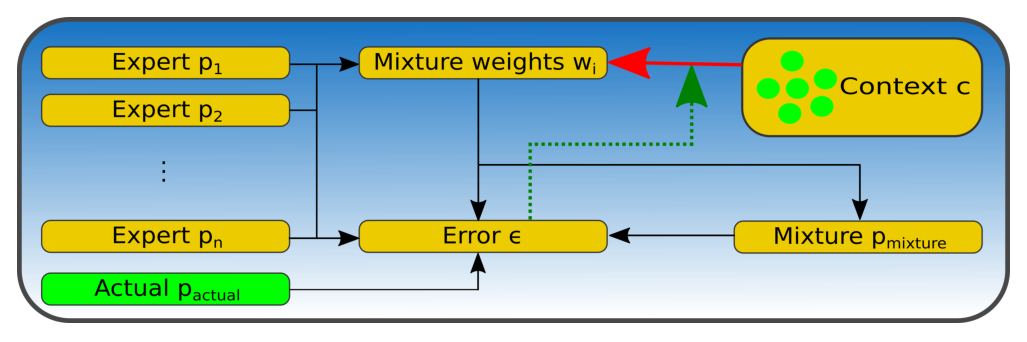
\includegraphics[width=\textwidth]{imgs/mix_of_experts.eps}
    \caption{Visualization of the network architecture of the context-sensitive mixture-of-experts online learning system. The red arrow indicates the learning connection, whereas the dotted green arrow indicates that the error signal is used to updated the weights of this connection using delta-rule learning.}\label{fig:data_example}
\end{figure}

There are two different possible variants to our mixture-of-experts online learning model.
One issue of such a learning system is that the actual position information of the target vehicle $p_{actual}$ and thus the error $\epsilon$ in eq.~\ref{eq:mixture_of_experts} is not available instantaneously but timely delayed.
Here, we show a first prototype that, for simplicity, ignores this delay issue and assumes that position information of the target vehicle $p_{actual}$ actually is available at prediction time.
In the future, we aim to investigate an online learning system that updates its weights $w_i$ once the error signal $\epsilon$ gradually becomes available.
However, the architecture of the model itself remains the same.
The only difference to the prototype shown here is the time when eq.~\ref{eq:mixture_of_experts} is applied to update the neural weights.
For the context-sensitive mixture-of-experts model, we use information about the current driving situation as identified in Sec.~\ref{subsubsec:eval_lstm} and Fig.~\ref{fig:histograms_on_board} as context $c$ for the learning system.
For the \emph{\ac{NGSIM}} data-set, we use the distance between the target-vehicle and the closest other vehicle as well as the number of surrounding relevant vehicles as context information.
Relevant means that those vehicles that are included in the \ac{SPA}-power representation are counted (see Sec.~\ref{subsubsec:encoding_schemes}).
For the \emph{On-board} data-set, the distance between the target and the ego-vehicle is additionally included in the context.

In this work, we employ the pre-trained \ac{LSTM} models using numerical inputs, the best-performing \ac{SPA}-power encoding scheme for each data-set, and a simple linear prediction as experts for our online learning prototype.
For training the model, we simulate online deployment by presenting the \ac{LSTM} models' predictions on the validation subsets to the system.
Thereby, the individual experts perform their prediction on previously unseen data samples.
We conduct individual simulation runs for each of both data-sets.

\section{Summary}
\label{sec:online_learn_summ}

